\chapter{Introduction}

In the realm of agriculture, the ability to efficiently detect and diagnose diseases in plants holds the key to 
improving agricultural practices and ultimately increasing crop yields.

\section{Project Objective}

Our project is dedicated to addressing this critical need by harnessing the power of Convolutional Neural 
Networks (CNNs). These neural networks are adept at learning intricate patterns and features from images, 
equipping them with the capability to distinguish between healthy and infected plants with remarkable precision.

\subsection{Practical Applications}

The potential applications of this project extend beyond traditional farming, as it can also be seamlessly 
integrated into daily life to care for indoor plants.

\subsection{Methodology Overview}

To accomplish our goal, we will undertake a comprehensive evaluation of two CNN models: one built from scratch 
and another utilizing pre-trained weights. Through a thorough analysis of various metrics, we aim to determine which 
model exhibits superior accuracy in plant disease detection, thereby contributing to the advancement of agricultural 
practices.

\section{Dataset Description}

For our project, we utilized the New Plant Diseases dataset, which is accessible at the following link: 
\url{https://www.kaggle.com/datasets/vipoooool/new-plant-diseases-dataset}.

This dataset has been generated by applying offline augmentation techniques to the original dataset, 
which is accessible on this GitHub repository: \url{https://github.com/spMohanty/PlantVillage-Dataset}.
The dataset comprises approximately 87,000 RGB images depicting both healthy and diseased crop leaves, 
categorized into 38 distinct classes. The complete dataset is partitioned into training and validation sets in 
an 80/20 ratio, while maintaining the original directory structure. Additionally, a separate directory containing 
5438 test images has been established for prediction purposes.

\subsection{Dataset Distribution}

\begin{table}[H]
	\centering
	\begin{tabularx}{1\textwidth}{>{\hsize=1.5\hsize\linewidth=\hsize}X
			>{\hsize=.5\hsize\linewidth=\hsize}X}
		\hline
		\textbf{Classes} & \textbf{Num. of images} \\
		\hline
		Strawberry\_\_healthy & 1824 \\
		Tomato\_\_healthy & 1926 \\
		Tomato\_\_Septoria\_leaf\_spot & 1745 \\
		Cherry\_(including\_sour)\_\_healthy & 1826 \\
		Potato\_\_healthy & 1824 \\
		Peach\_\_Bacterial\_spot & 1838 \\
		Grape\_\_Black\_rot & 1888 \\
		Tomato\_\_Tomato\_mosaic\_virus & 1790 \\
		Tomato\_\_Leaf\_Mold & 1882 \\
		Strawberry\_\_Leaf\_scorch & 1774 \\
		Tomato\_\_Late\_blight & 1851 \\
		Corn\_(maize)\_\_healthy & 1859 \\
		Squash\_\_Powdery\_mildew & 1736 \\
		Tomato\_\_Early\_blight & 1920 \\
		Grape\_\_healthy & 1692 \\
		Cherry\_(including\_sour)\_\_Powdery\_mildew & 1683 \\
		Pepper,\_bell\_\_healthy & 1988 \\
		Peach\_\_healthy & 1728 \\
		Tomato\_\_Tomato\_Yellow\_Leaf\_Curl\_Virus & 1961 \\
		Apple\_\_healthy & 2008 \\
		Potato\_\_Late\_blight & 1939 \\
		Corn\_(maize)\_\_Northern\_Leaf\_Blight & 1908 \\
		Pepper,\_bell\_\_Bacterial\_spot & 1913 \\
		Grape\_\_Leaf\_blight\_(Isariopsis\_Leaf\_Spot) & 1722 \\
		Raspberry\_\_healthy & 1781 \\
		Apple\_\_Cedar\_apple\_rust & 1760 \\
		Corn\_(maize)\_\_Common\_rust\_ & 1907 \\
		Soybean\_\_healthy & 2022 \\
		Tomato\_\_Bacterial\_spot & 1702 \\
		Potato\_\_Early\_blight & 1939 \\
		Grape\_\_Esca\_(Black\_Measles) & 1920 \\
		Tomato\_\_Target\_Spot & 1827 \\
		Apple\_\_Apple\_scab & 2016 \\
		Apple\_\_Black\_rot & 1987 \\
		Corn\_(maize)\_\_Cercospora\_leaf\_spot\_Gray\_leaf\_spot & 1642 \\
		Tomato\_\_Spider\_mites\_Two-spotted\_spider\_mite & 1741 \\
		Orange\_\_Haunglongbing\_(Citrus\_greening) & 2010 \\
		Blueberry\_\_healthy & 1816 \\
		\hline
	\end{tabularx}
	\caption{Number of images for each class of the training set}	
		
\end{table}

\begin{figure}[H]
    \centering
    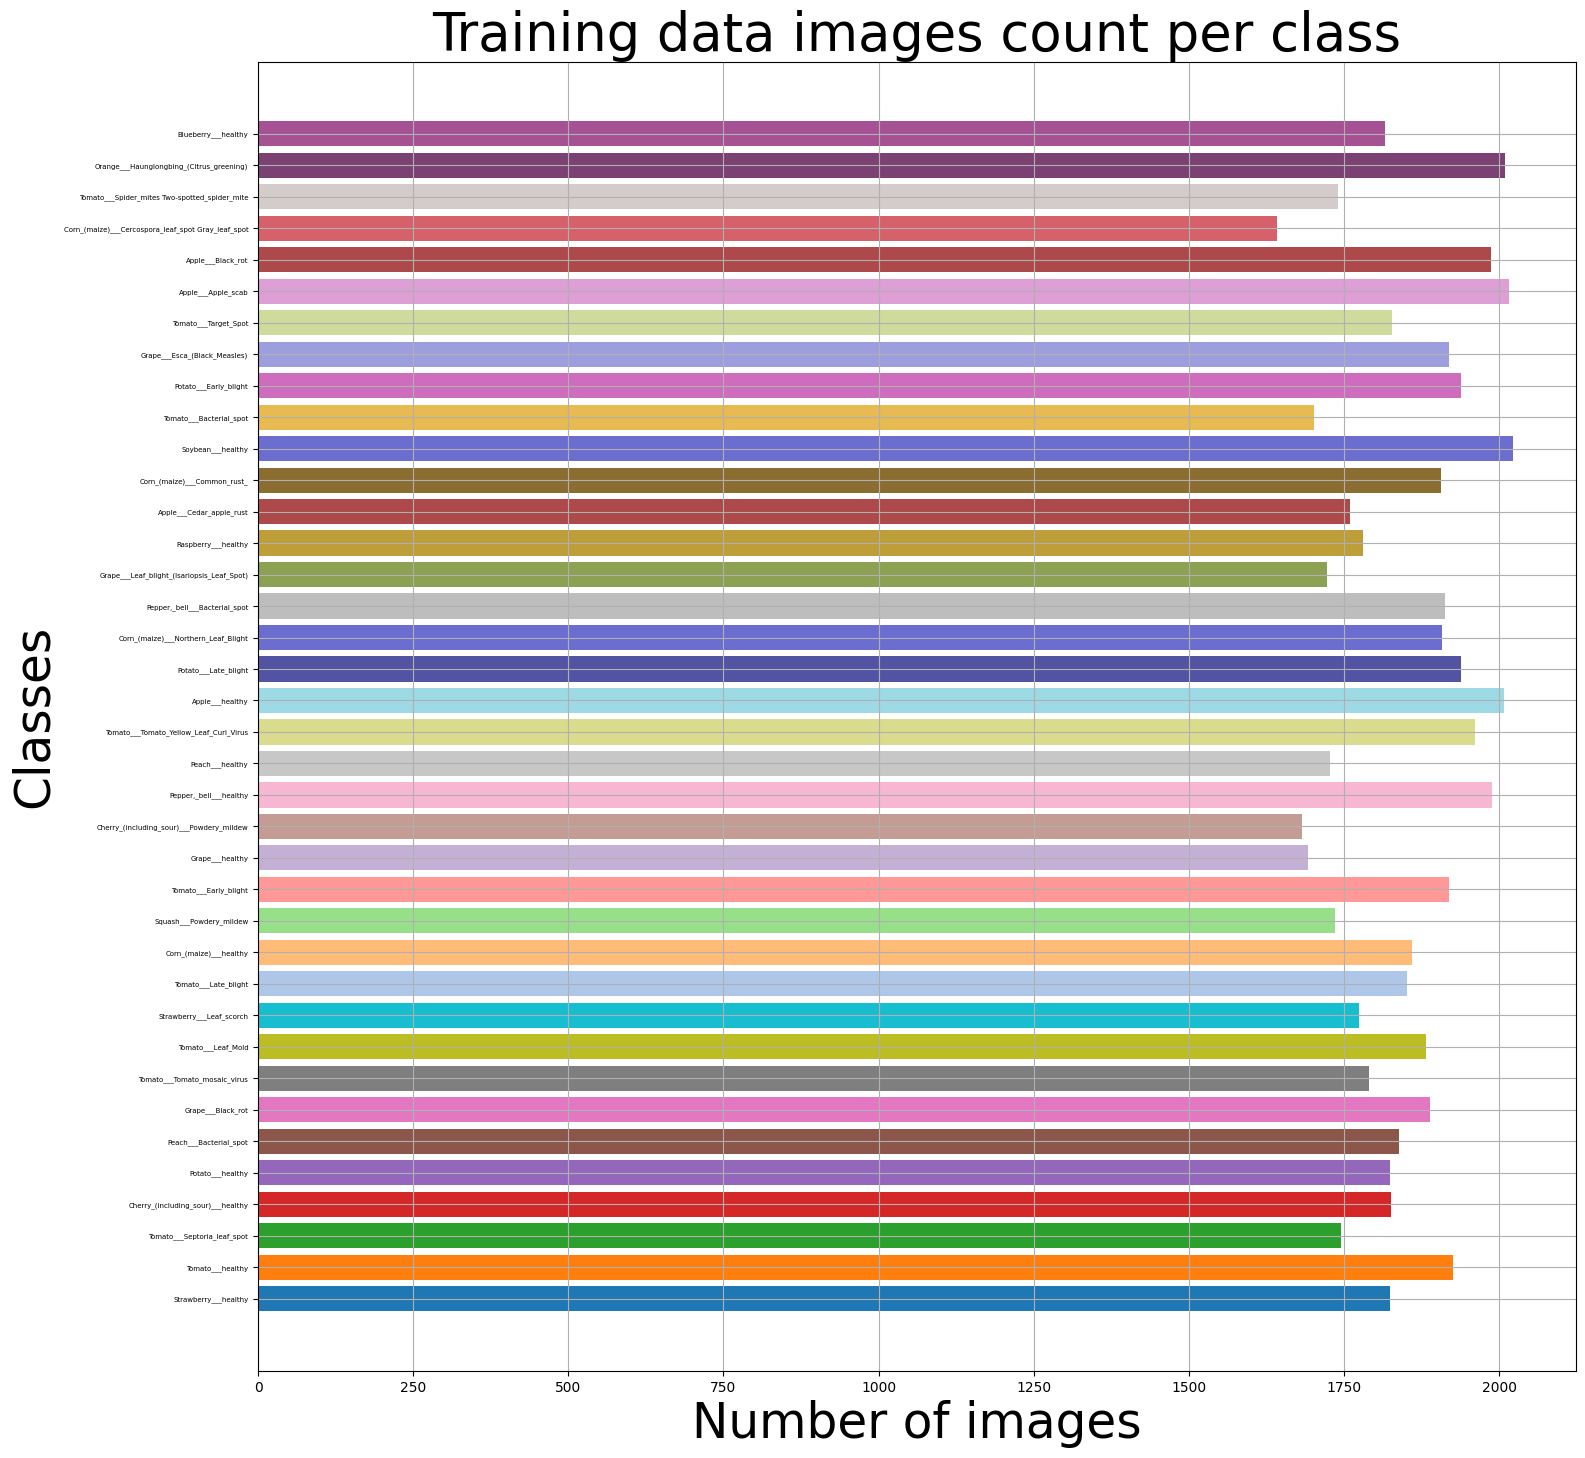
\includegraphics[width= 0.9\textwidth]{assets/class_distribution_big_leaves.png} 
    \caption{Class distribution} 
    \label{fig:immagine}
\end{figure}

As we can see the class distribution of the training dataset is quite balanced.
